\documentclass[12pt]{article}
\usepackage{sydewkrpt}
\usepackage{longtable}
\usepackage{array}
\usepackage{ragged2e}
\usepackage{amsmath}
\usepackage{amssymb}
\usepackage{float}
\usepackage[toc]{glossaries}
\usepackage[toc,page]{appendix}
\usepackage{listings}
\usepackage{pdfpages}

\newcolumntype{P}[1]{>{\RaggedRight\hspace{0pt}}p{#1}}

\newenvironment{conditions*}
  {\par\vspace{\abovedisplayskip}\noindent\begin{tabular}{>{$}l<{$} @{${}={}$} l}}
  {\end{tabular}\par\vspace{\belowdisplayskip}}

\clubpenalty = 10000
\widowpenalty = 10000
\displaywidowpenalty = 10000

%%%%%%%%%%%%%%%%%%%%%%%%%%%%
%%%    Begin Document    %%%
%%%%%%%%%%%%%%%%%%%%%%%%%%%%
\begin{document}
\pagenumbering{roman}

\waterlootitle{Two-Stage \& Chance Constrained Stochastic Programming Option Portfolio Optimization Using Binomial Tree Pricing\\}{
  SYDE 531: Final Project
}{
  D. Scott Neil -- 20349210\\
  Matthew Chong -- 20341648\\
}

%\dotableofcontents

\newpage 
\doublespacing
\pagenumbering{arabic}
\setlength{\parindent}{1cm}

\section{Introduction}
The stock market involves the buying and selling of ownership (shares) of a public company.  There is an agreed upon price with which the trade is executed, and is eventually settled through an exchange (TSX, NASDAQ, etc.).  However, the stock market is just one aspect of the entire capital market. The derivatives market, for example, consists of financial instruments that are derived from other forms of securities (stocks, bonds, futures).  One of the better-known instruments is the option since one of the underlying assets is a stock. For the scope of this report the authors will focus solely on options.

A stock option can be very beneficial to any sophisticated portfolio. It is essentially ``a contract that gives the buyer the right, but not the obligation, to buy or sell [a stock] at a specific price on or before a certain date.'' \cite{volatility}. The buyer must purchase the option at a price outlined in the options market. In brief, someone is selling you a right, which means the buyer must also pay a premium to enter in the contract. For the purpose of this report the researchers will use European Options, which are options that can only be exercised on the expiry date \cite{euro_option}. 

Pricing of European options has been a well researched topic. The most widely accepted method is the use of the Black-Scholes formula. Based on the properties of the underlying asset the formula determines a theoretical fair price of the option at that specific moment in time. However, the formula does not take into account the randomness of the underlying stock price movement. The Binomial Tree Pricing Theory allows an investor to assign a probability to the movement of a stock price and then calculate the fair price of an option for any market condition. 

For this project, the Jarrow-Rudd binomial pricing model is used, which assumes equal probability for each movement in stock price \cite{jarrow1983option, jrudd_other, jrudd_impl}. An example of a binomial tree can be found in \ref{fig:bin_tree}. Each level represents a time period moving from one state to another. The nodes in the tree are the option price for a given a set of market conditions. The probabilities denoted by p, are the probabilities of the market moving to that state. Nodes that have more paths that lead to them are more likely to occur and therefore have higher probabilities of occurring. The randomness is then associated with the unknown movement of the market and consequently the underlying assets.
 
 \begin{figure}[H]
  \begin{centering}
    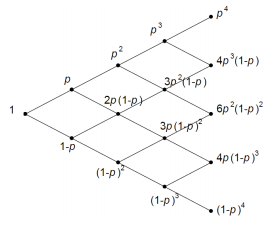
\includegraphics[scale=1.0]{bin_tree.png}
    \caption{4-Stage Binomial Tree Example \cite{bin_tree}}
    \label{fig:bin_tree}
  \end{centering}
\end{figure}
 
Portfolio optimization is the process of choosing the proportions of various assets to help improve a portfolio based on certain criterion. The criterion is combined directly or indirectly with considerations like the expected value of the portfolio’s rate of return, returns variability and other measures of financial risk. The goal of portfolio optimization is to reduce the risk an investor takes on while trying to maximize profit with an uncertainty of market conditions.

Portfolios are constructed using Stochastic Programming, obtaining scenarios from the binomial trees of each option. Two methods are used: Two-Stage and Chance Constraints. Two-Stage programming creates a scenario for each possible outcome of the market and weights each of these by their associated likelihood of occurrence. Penalties are added when a specific scenario fails to meet the desired target. Chance Constraints aim to meet the highest target return possible at a given reliability. The reliability is set prior to optimizing and desired target found in the process. Section \ref{sec:two_opt_port} contains results and a discussion of each of the methods.


\section{Objective}
To create an optimal portfolio of two independent options, priced using the Jarrow Rudd binomial model \cite{jarrow1983option, jrudd_other, jrudd_impl}, with the two-stage stochastic programming method.

\section{Assumptions}
The following assumptions were made to reduce the complexity of the design problem:
\begin{itemize}
	\item The time period to calculate volatility is from November 1, 2012 to January 1, 2013
	\item The initial stock price is taken at January 1, 2013 (time = 0)
	\item Time to maturity of option is 6 months or 1 year, and each time period is 4 months
	\item The risk free interest rate is 3\%
	\item The stock movements have equal probability of moving up or down
	\item Use of European options that can only be exercised at maturity
	\item Movement of each asset is independent of each other
\end{itemize}


\section{The Model}
\subsection{Design Variables}
The design variables for the problem are as follows:
\begin{itemize}
	\item The number of option contracts to purchase for each security (both methods)
	\item Surplus and Deficit penalties for each scenario, activated when the $target$ is not met (in Two-Stage)
	\item Target (in Chance Constrained)
\end{itemize}

\newpage
\subsection{Two-Stage Stochastic Programming Problem}

\begin{equation*}
\label{eqn:opt_opt1}
\begin{aligned}
& \text{maximize}
& \text{target} - \sum_{i=0}^{n} \pi_{i}  (P^i) - \theta \sqrt{var(P)}\\
& \text{subject to}\\
& & \sum_{j=0}^{2} price_j  x_j = \text{budget} \\
& & c_{1}^{i} x_{1} + c_{2}^{i} x_{2} + S^{i} - D^{i} = \text{target} \\
& & x_j \geq 0
\end{aligned}
\end{equation*}
Where:
\begin{conditions*}
P^i & $(P_{s} S^{i} - P_{d} D^{i})$ \\
var(P) & $\sum_{i=0}^n \pi_{i} (P^i - \overline{P})^2$ \\
budget & the total allowable dollar value to allocate between options \\
target & the budget multiplied by expected return  (\%) \\
price_j & price of one option contract of option $j$ \\
S^{i} & surplus penalty for $i^{th}$ scenario \\
D^{i} & deficit penalty for $i^{th}$ scenario \\
c^{i}_{j} & expected return for scenario $i$ for option $j$ \\
\pi^i & penalty weighting for scenario $i$ (represents likelihood of occurrence) \\
\theta & weight placed on variance of penalty terms
\end{conditions*}

\subsection{Chance Constrained Stochastic Programming Problem}

\begin{equation*}
\label{eqn:opt_opt2}
\begin{aligned}
& \text{maximize} 
& \text{target} \\
& \text{subject to}\\
& \sum_{j=0}^{2} price_j  x_j = \text{budget} \\
& \overline{c_{1}} x_{1} + \overline{c_{2}} x_{2} - \beta \sqrt{x^T \text{Cov}(c_1, c_2) x} \geq \text{target} \\
& x_j \geq 0
\end{aligned}
\end{equation*}
Where:
\begin{conditions*}
budget & the total allowable dollar value to allocate between options \\
price_j & price of one option contract of option $j$ \\
\overline{c_{i}} & mean expected return for option $i$ \\
\beta & evaluation of reliability percentage, $\alpha$ (set prior to optimization), on $N(0,1)$ \\
\end{conditions*}

\section{Simulating Option Prices}
The set up of the problem begins with the design of the binomial trees. The complexity of the problem stems from the number of time periods and not the number of assets used. For this reason only 2 assets were chosen; BMO.TO and PFE. The number of time periods that was chosen was 4, yielding 5 leafs in each tree and giving rise to 25 possible scenarios. 

\newpage
To build the Jarrow-Rudd tree the underlying asset's information used can be found in Table~\ref{tab:thetable}.

\begin{table}[H]
	\centering
    \begin{tabular}{|l|l|l|}
    \hline
    ~                                 & BMO.TO & PFE   \\ \hline
    Initial Stock Price (Jan 1, 2013) & 57.90  & 24.87 \\ \hline
    Strike Price                      & 60     & 28    \\ \hline
    Volatility                        & 9\%    & 12\%  \\ \hline
    Time to Maturity (months)         & 12     & 12    \\ \hline
    Risk-Free Interest Rate           & 3\%    & 3\%   \\ \hline
    \end{tabular}
    \caption {Asset and Option Details}
    \label{tab:thetable}
\end{table}


The volatility for each asset was calculated using the annualized volatility (adapted from \url{https://gist.github.com/johntyree/4587049}). The strike price was chosen arbitrarily, but  also to represent an actual option contract.

	Using the implementation by Sanjiv Das and Brian Granger \cite{jrudd_impl}, seen in $binomial\_tree.py$, a pricing method is build, which yields two trees for each asset. One tree is the fair option price for each state, and the other tree is the predicted stock price for each state. Based on the given information, the expected return for each scenario is calculated using Equation~\eqref{eq:expreturn}.

\begin{equation}\label{eq:expreturn}
	Return = max((p_{Ni} - p_s) - p_{opt}, -p_{opt})
\end{equation}
Where:
\begin{conditions*}
p_{Ni} & price in the last time period of the $i_{th}$ \\
p_s & strike price \\
p_{opt} & price of one option contract \\
\end{conditions*}

\section{Two-Option Portfolio}
\label{sec:two_opt_port}
A two option portfolio was tested and modified to learn how to implement two-stage stochastic programming and understand how it operates. The next section outlines the starting conditions and parameters used in the optimization. In later section, these parameters are tweaked and results discussed.

\subsection{Two-Stage Stochastic Programming}
Table~\ref{tab:init_cond} specifies the initial conditions for the optimization procedure.

\begin{table}[H]
	\centering
    \begin{tabular}{|l|l|}
    \hline
    	\textbf{parameter} & \textbf{value} \\ \hline
    	budget & \$1000 \\ \hline
	desired ROI & 10\% \\ \hline
	target & \$1100 \\ \hline
	$P_s$ & 0.01 \\ \hline
	$P_d$ & 0.01 \\ \hline
	$\theta$ & 0.5 \\ \hline
	time to maturity & 6, 12 \\ \hline
	periods & 4 \\ \hline
    \end{tabular}
    \caption {Initial conditions}
    \label{tab:init_cond}
\end{table}

\subsubsection{Results}
The optimal result is found in Table~\ref{tab:result_pen}.
The surplus and deficit terms are not included, but rather the overall penalty and standard deviation are shown for simplicity (there are 25 scenarios and they do not all need to be listed).
Also, the number of contracts for each security has been rounded to the nearest whole contract, as you cannot purchase a partial contract.

\begin{table}[H]
	\centering
    \begin{tabular}{|l|l|l|}
    \hline
    	~ & \textbf{12-month} & \textbf{6-month} \\ \hline
    	obj\_fun value & 1102.60 & 1101.50 \\ \hline
	BMO.TO & 385 & 865 \\ \hline
	PFE & 586 & 1043 \\ \hline
	total pentaly & 10.70 & 10.85 \\ \hline
	$\sigma_{penalty}$ & 16.18 & 18.71 \\ \hline
    \end{tabular}
    \caption {12- \& 6-month horizon portfolios}
    \label{tab:result_pen}
\end{table}

\subsubsection{Discussion}

Multiple parameters within the optimization were altered during testing, and it was found that, in general, impact on the results were minimal. Firstly, changing the penalty weights, $P_s$ and $P_d$, only changed the objective function value, not allocation between assets. Multiple values, such as 0.01, 0.5, 1.0, were tested and all resulted in the same outcome. Making the values different was also attempted, as a surplus in return is more favourable than a deficit, but this caused the penatly terms to increase greatly (to multi-million values). The optimization procedure either does not complete successfully due to the parameter matrix becoming singular (if difference in penalty weights is relatively large), or simply results in extremely large total penalty, standard deviation, and design variable values (if difference is relatively small). We’re unsure why this is occurring, so reverted to having these parameters equal.

Next, the problem was tested with and without the variance term in the objective function. It was found that adding this term has no impact on the allocation. The researchers again are unsure why this is the case, but even with testing multiple values of $\theta$ similar results were observed. It does affect the objective function value, as expected, but does not alter any of the design parameter values.
	
Additionally, we initially observed that in each scenario, the difference between the surplus and deficit parameters is essentially zero, but their values are quite large. It was then determined that a constraint was needed on each of these parameters to ensure their values were greater than, or equal to, zero. This shifted the penalty all to one term, as it should, which altered the allocation of assets in both portfolios.
	
Lastly, it is seen in the results table that there is minimal difference between the 6- and 12-month portfolios. We expected this and included the two scenarios to test the robustness of the problem formulation. If these results were vastly different, it would be due to an error in either the pricing scheme (i.e. binomial tree) or optimization problem. Corrections could then be made as needed and portfolios reconstructed.

\subsection{Chance Constrained Stochastic Programming}
The other method that was investigated was using the chance constraint method. The chance constraint method for this particular problem involves assigning a reliability term that asserts we maximize our target for a given probability. Assuming our allocations are random the chance constrained formulation is shown below:

Table~\ref{tab:init_cond2} shows the initial conditions of the chance constrained optimization similar to the two-stage stochastic programming optimization.

\begin{table}[H]
	\centering
\begin{tabular}{|l|l|}
\hline
	\textbf{parameter} & \textbf{value} \\ \hline
	budget & \$1000 \\ \hline
	time to maturity & 6\\ \hline
	periods & 4 \\ \hline
\end{tabular}
\caption {Initial conditions}
\label{tab:init_cond2}
\end{table}

\subsubsection{Results}
The optimization was run using different reliability methods in the attempt to produce the best results. Table~\ref{tab:result_cc} shows the corresponding optimizations. 

\begin{table}[H]
\centering
\begin{tabular}{|l|l|l|l|}
\hline
	~ & \textbf{30\% Reliability} & \textbf{62.15\% Reliability} & \textbf{90\% Reliability} \\ \hline
	obj\_fun value & 6057 & 0.82 & -2837 \\ \hline
	BMO.TO & 0 & 0 & 993 \\ \hline
	PFE & 8093 & 8093 & 0\\ \hline
\end{tabular}
\caption {Varying Reliability Portfolios}
\label{tab:result_cc}
\end{table}

\subsubsection{Discussion}
Based on the results, it was found that the optimization did not perform well. If these two securities constituted the entire portfolio, a ``break even'' return is only observed at a rate of approximately 62\%. The maximization was very sensitive to changes in the reliability and as such the allocations varied significantly too. With an increased reliability, the objective function would actually yield a negative return, which is not desireable. Conversely, the optimization would only produce positive returns when the reliability was below 62\%. 

The results can be explained due to the simplicity of the portfolio.
Only considering two assets and four time periods results in a limited number of outcomes.
Additionally, neither of these options are good investments; both assets only have positive returns in their uppermost scenarios, with BMO.TO also producing a positive return at its second highest.
The average return for BMO.TO is 0.78 and PFE is 0.27, and variance of BMO.TO is 8.09 and PFE 0.81 -- on average, neither asset will return the initially invested capital.
It is therefore very difficult to establish a well performining portfolio with this limited universe and poor performing assets.
This is discussed in the following sections and it is recommended that a more diversified portfolio be considered.


\section{Comparison of Methods}
Comparing the methods between the Two-Stage Stochastic Programming and Chance Constrained methods there are a few conclusions that can be made. One observation is that the Two-Stage method produced positive returns regardless of the time horizon, while the Chance Constrained method was binary producing only positive returns if it was below the threshold reliability of 62.15\%. This is due to the fact that in the Two-Stage method there is a penalty associated with not meeting the desired return so the optimization attempts to reduce that penalty. The Chance Constrained method however has no penalty associated with not meeting the return, but instead attempts to maximize the target while maintaining a specified reliability. For this reason, the method can have negative returns, while maintaining reliability. Also the Chance Constrained method does not consider each potential scenario individually, but uses averages instead. Information is lost by doing this, which may contribute to its weaker performance.

Another observation made is that the Two-Stage method allocates the budget in a more even manner compared to the Chance Constrained method. 
One hypothesis is that the assets may not compliment each other well and this is exposed more in the Chance Constrained method. 
Another cause could be due to differences in variance of price or payoff of the assets. In this example, BMO.TO has positive returns in two of the five scenarios, where as PFE only in one. Therefore allocating all to BMO.TO in cases of high reliability is understandable as their are more opportunities to make positive returns and therefore maximize return (or in this case minimize losses).
Ultimately, neither of these assets are strong performers and increasing the number and diversity would have much different results and should be investigated.

\section{Recommendations and Conclusions}
Further improvements can be made to make this optimization problem yield better results. Changes to gathering the data in terms of choosing different time periods, will have a direct impact on the performance of the strategy. Certain time periods could be much more volatile for specific stocks due to external economic factors. 

In addition, when choosing the stocks to be used in the portfolio, one key term that should be taken into account is diversification. The United States Securities and Exchange Commission describes diversification as follows: “The practice of spreading money among different investments to reduce risk is known as diversification. By picking the right group of investments, you may be able to limit your losses and reduce the fluctuations of investment returns without sacrificing too much potential gain.” \cite{diversity}.  One example of why diversification is required is to reduce industry specific risk. If a portfolio is only made up of technology stocks, and the technology industry is hit with increase costs in silicon or net neutrality, then the entire sector is affected. Therefore, the entire portfolio is dictated solely by the industry. If the portfolio is diversified, and one industry is doing poorly another industry could be doing well thereby hedging the positions one takes. Choosing more assets from different industries could have significant effects on how the strategy performs, including increasing complexity, so it is important to note that making any of these changes could yield completely different outcomes.

In addition, many of the parameters were arbitrary. Looking more into determining the risk-free interest rate, actual strike prices from the Chicago Board Options Exchange, and even incorporating dividend payments would have significant impacts on how the option is priced. 
	
Going forward, applications can be built off of this optimization carried out in this report. One such application is through the use of Arrow-Debreu Securities to create a riskless portfolio. Arrow-Debreu Securities have similar characteristics to that of a binomial option tree in that they have a specified payoff for a specific state in the market \cite{tirole2010theory, AD_secs}. These securities allow for a riskless portfolio by hedging securities off of one another to create an equilibrium. One can theoretically calculate the payoff of a portfolio using a linear combination of all securities. Given a makeup of securities using the optimization techniques presented in this report, different types of securities (stocks, bonds, futures etc) can be introduced to a portfolio and optimized to yield the best payoff.
	
Lastly, the method of binomial trees for pricing options is likely not the most accurate model. One change could be the introduction of trinomial trees. These have three transitions: up, down, or neutral. This may better represent movements of securities, but improvements would need to be tested. Research has also been conducted in the use of Stochastic Programming for pricing options, using scenario trees \cite{stoc_prog_option}. These again are similar to binomial trees, but have $n$ transitions to the next stage from each state, making the model potentially much more complex (and increasing scenarios greatly), but also more accurate. Improvements again would need to be tested to understand if the increased pricing accuracy is worth the added complexity.

In conclusion, these two methods are powerful for calculating optimal portfolios, but further research needs to be conducted. Increasing the number of assets, time periods, and diversity (in terms of sector and asset class) should be investigated. Additionally, alternative option pricing methods should be tested and their accuracy compared against actual prices. Both of these will increase the complexity of the problem, but will generate more meaningful results and combine to formulate a more accurate representation of portfolio construction and financial markets.


\newpage
\addcontentsline{toc}{section}{References}

\bibliographystyle{IEEEtran}

\bibliography{bib}

\newpage
\begin{appendices}
\section{Implementation} \label{ap:code}
\subsection{Binomial Tree}
\lstinputlisting[language=Python]{binomial_tree.py}

\subsection{Option Class}
\lstinputlisting[language=Python]{option.py}

\subsection{Optimization Procedures}
\includepdf[pages={-}]{OptimizationPythonNotebook.pdf}
\end{appendices}
\end{document}
